\section{Why Workflows}

%%%%%%%%%%%%%%%%%%%%%%%%%%%%%%%%%%%%%%%%%%%%%%%%%%%%%%%%%%%%%%%%%%%%%%%%%%%%%%%%
\begin{frame}
    \frametitle{Outline}
    \begin{columns}[t]
        \begin{column}{.5\textwidth}
            \tableofcontents[sections={1-9},currentsection]
        \end{column}
        \begin{column}{.5\textwidth}
            \tableofcontents[sections={10-18},currentsection]
        \end{column}
    \end{columns}
\end{frame}

%%%%%%%%%%%%%%%%%%%%%%%%%%%%%%%%%%%%%%%%%%%%%%%%%%%%%%%%%%%%%%%%%%%%%%%%%%%%%%%%
\begin{frame}
  \frametitle{What is this about?}
   \question[Questions]{\begin{itemize}
                         \item I can code everything! Can I?
                         \item What is the benefit of a workflow system?
                         \item What distinguishes a workflow system from a ``pipeline''?
                        \end{itemize}
                       }
   \docs[Objectives]{\begin{enumerate}
                      \item Introducing workflow engines (particularly \texttt{Snakemake})!
                     \end{enumerate}}
\end{frame}  

%%%%%%%%%%%%%%%%%%%%%%%%%%%%%%%%%%%%%%%%%%%%%%%%%%%%%%%%%%%%%%%%%%%%%%%%%%%%%%%%
\begin{frame}
  \frametitle{Data Analysis}
  \begin{onlyenv}<1| handout:0>
    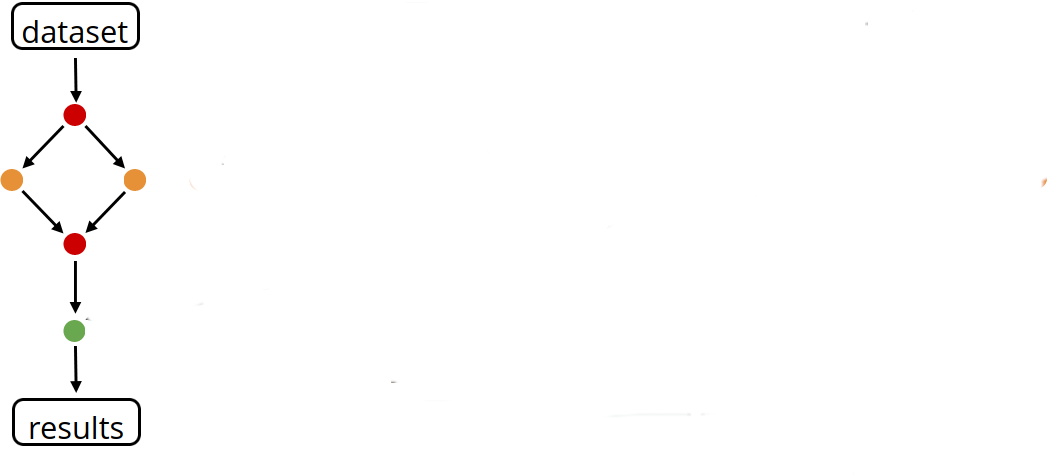
\includegraphics{snakemake/analysis_1.png}
    
\includegraphics{snakemake/phd_left.png}
  \end{onlyenv}
  
  \begin{onlyenv}<2| handout:1>
    \includegraphics{snakemake/analysis_2.png}
    
\includegraphics{snakemake/phd_full.png}
  \end{onlyenv}
\end{frame}
